%!TEX root = ../Thesis.tex
\chapter{Numerical Analysis} \label{ch:numerical-analysis}
\epigraph{``\itshape{A computer lets you make more mistakes faster than any invention in human history - with the possible exceptions of handguns and tequila.}"}{--- \textup{Mitch Ratliffe}, Technology Review, April 1992}

Some systems can be solved analytically in terms of time-dependent coordinates. Other systems are non-linear and the vast majority cannot be solved analytically. This is the case for the restricted three-body problem, \crefrange{eq:H-x}{eq:H-py}. To solve these equations of motion, we must use numerical methods.

The simplest numerical integration is the first order linear approximation known as the Euler method. There are three variants of the Euler method: explicit, implicit and symplectic. As we will see, the explicit Euler will typically increase the energy, implicit Euler will decrease the energy and the symplectic Euler will oscillate the energy slightly but on average conserve pretty well.

We will now solve the restricted three-body problem equations of motion, \crefrange{eq:H-x}{eq:H-py}. First we discretize the equations with a linear approximation:

\begin{align}
\Delta x &= +\dfrac{\partial H}{\partial p_x}\Delta t = (p_x + y)\Delta t, \\[0.2cm]
\Delta y &= +\dfrac{\partial H}{\partial p_y}\Delta t = (p_y - x)\Delta t, \\[0.2cm]
\Delta p_x &= -\dfrac{\partial H}{\partial x}\Delta t = \left(p_y - \dfrac{(1-k)(k+x)}{((k+x)^2+y^2)^{3/2}} + \dfrac{k(1-k-x)}{((1-k-x)^2+y^2)^{3/2}}\right)\Delta t, \\[0.2cm]
\Delta p_y &= -\dfrac{\partial H}{\partial y}\Delta t = \left(-p_x - \dfrac{(1-k)y}{((k+x)^2+y^2)^{3/2}} - \dfrac{k y}{((1-k-x)^2+y^2)^{3/2}}\right)\Delta t.
\end{align}

From now on we will use $h$ instead of $\Delta t$ for the time step size.

\section{Explicit Euler algorithm}
All new values $(x,y,p_x,p_y)_{i+1}$ refer to known values from the previous time step $(x,y,p_x,p_y)_i$.
\begin{align}
x_{i+1} &= (p_{x,i} + y_i)h + x_i, \\[0.2cm]
y_{i+1} &= (p_{y,i} - x_i)h + y_i, \\[0.2cm]
p_{x,i+1} &= \left(p_{y,i} - \dfrac{(1-k)(k+x_i)}{((k+x_i)^2+y_i^2)^{3/2}} + \dfrac{k(1-k-x_i)}{((1-k-x_i)^2+y_i^2)^{3/2}}\right)h + p_{x,i}, \\[0.2cm]
p_{y,i+1} &= \left(-p_{x,i} - \dfrac{(1-k)y_i}{((k+x_i)^2+y_i^2)^{3/2}} - \dfrac{k y_i}{((1-k-x_i)^2+y_i^2)^{3/2}}\right)h + p_{y,i}.
\end{align}

\section{Implicit Euler algorithm}
Same as explicit Euler, except that all variables on the right-hand side refers to variables in the current time step, $i+1$. This algorithm would involve finding four roots simultaneously and numerically. Since we know the symplectic to be more correct, we skip the implicit Euler (formula included in appendix \ref{app:implicit_euler}).

\section{Symplectic Euler algorithm}
This algorithm manifests as a mixture between explicit and implicit Euler. New values of $(x,y)_{i+1}$ refer to unknown values from the same time step $(x,y,p_x,p_y)_{i+1}$ but all new values of $(p_x,p_y)_{i+1}$ refer only to known values from the previous time step $(x,y,p_x,p_y)_i$:
\begin{align}
x_{i+1} &= (p_{x,i+1} + y_{i+1})h + x_i \label{eq:euler-s-x}, \\[0.2cm]
y_{i+1} &= (p_{y,i+1} - x_{i+1})h + y_i \label{eq:euler-s-y}, \\[0.2cm]
p_{x,i+1} &= \left(p_{y,i} - \dfrac{(1-k)(k+x_i)}{((k+x_i)^2+y_i^2)^{3/2}} + \dfrac{k(1-k-x_i)}{((1-k-x_i)^2+y_i^2)^{3/2}}\right)h + p_{x,i} \label{eq:euler-s-px}, \\[0.2cm]
p_{y,i+1} &= \left(-p_{x,i} - \dfrac{(1-k)y_i}{((k+x_i)^2+y_i^2)^{3/2}} - \dfrac{k y_i}{((1-k-x_i)^2+y_i^2)^{3/2}}\right)h + p_{y,i}. \label{eq:euler-s-py}
\end{align}
As opposed to implicit Euler, this can easily be solved by solving \eqref{eq:euler-s-x} and \eqref{eq:euler-s-y} for $x_{i+1}$ and $y_{y+1}$
\begin{align}
x_{i+1} &= \dfrac{x_i + h(h p_{y,i+1} + p_{x,i+1} + y_i)}{1+h^2}, \label{eq:euler_s_x2} \\[0.5cm]
y_{i+1} &= \dfrac{y_i - h(h p_{x,i+1} - p_{y,i} + x_i)}{1+h^2}, \label{eq:euler_s_y2}
\end{align}
and then we can run the algorithm in the order \eqref{eq:euler-s-px}, \eqref{eq:euler-s-py}, \eqref{eq:euler-s-x} and \eqref{eq:euler-s-y}.

\section{First Test Runs with First-Order Euler Methods}
The explicit and symplectic Euler algorithm was implemented in Python. The first two things we want to investigate are:
\begin{enumerate}
    \item Does the trajectories look like we expect them to? 
    \item Is the Hamiltonian conserved?
\end{enumerate}
For symplectic integrators the trajectories look like we expect them to (see \ref{fig:r3b_symplectic_euler}), but not for the non-symplectic explicit Euler (see \ref{fig:r3b_explicit_euler}). The Hamiltonian is not conserved for either first order (Euler) Methods, but $H$ for the symplectic Euler was conserved on average over an orbit in a closed orbit.
The simulations in Figure \ref{fig:r3b_explicit_euler} \ref{fig:r3b_symplectic_euler} was run with the following parameters:
\begin{adjustwidth*}{0cm}{-0.4cm}
\begin{lstlisting}[language=Python,caption={Initial conditions, step size and duration for initial test run},label={lst:testrun}]
# Duration and step size
DURATION = 1.5*(2*np.pi)
H = 0.0001

# Initial Conditions
X0=0.5
Y0=0.2
PX0=0
PY0=0.5
\end{lstlisting}
\end{adjustwidth*}

\begin{figure}
    \centering
        \subbottom[Explicit Euler $(\mathscr{X},\mathscr{Y})$ trajectory. Earth in origin, moon orbit in grey, first half of spacecraft trajectory is red, last half is blue.]{
            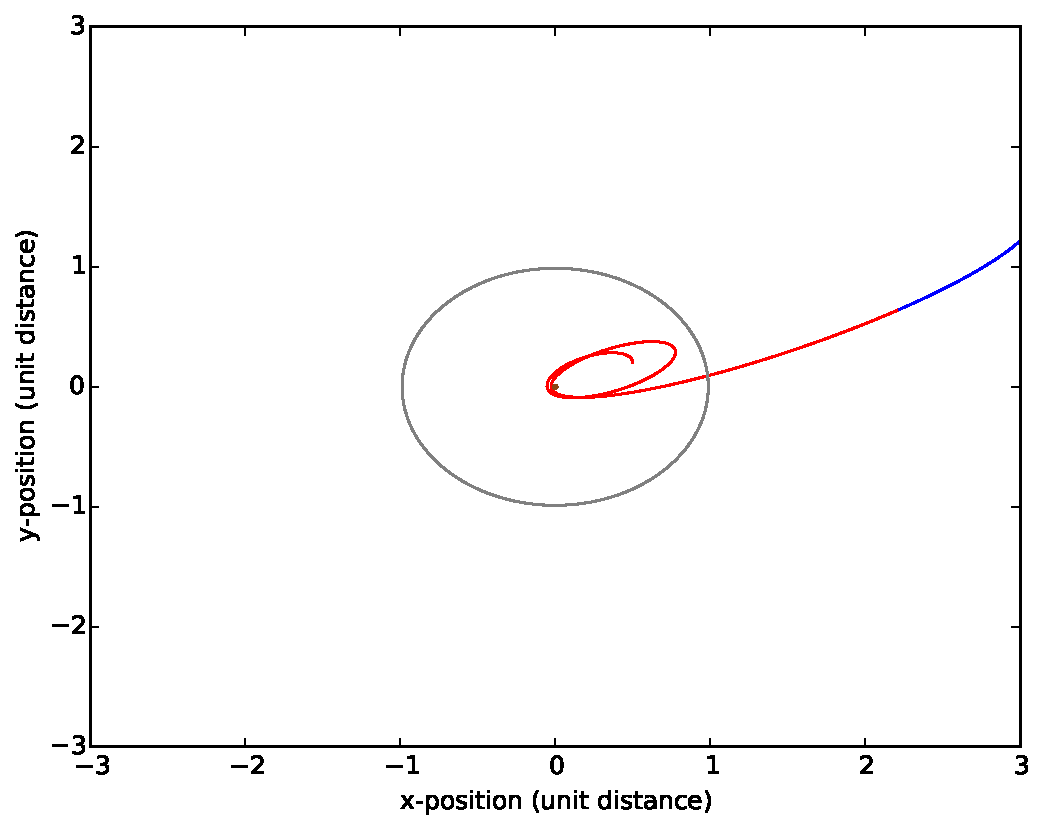
\includegraphics[scale=0.41]{fig/r3b-testing/r3b_y(x)_euler_explicit.pdf}
            \label{fig:r3b_y(x)_euler_explicit}
        }
        \subbottom[Explicit Euler $H(t)$.]{
            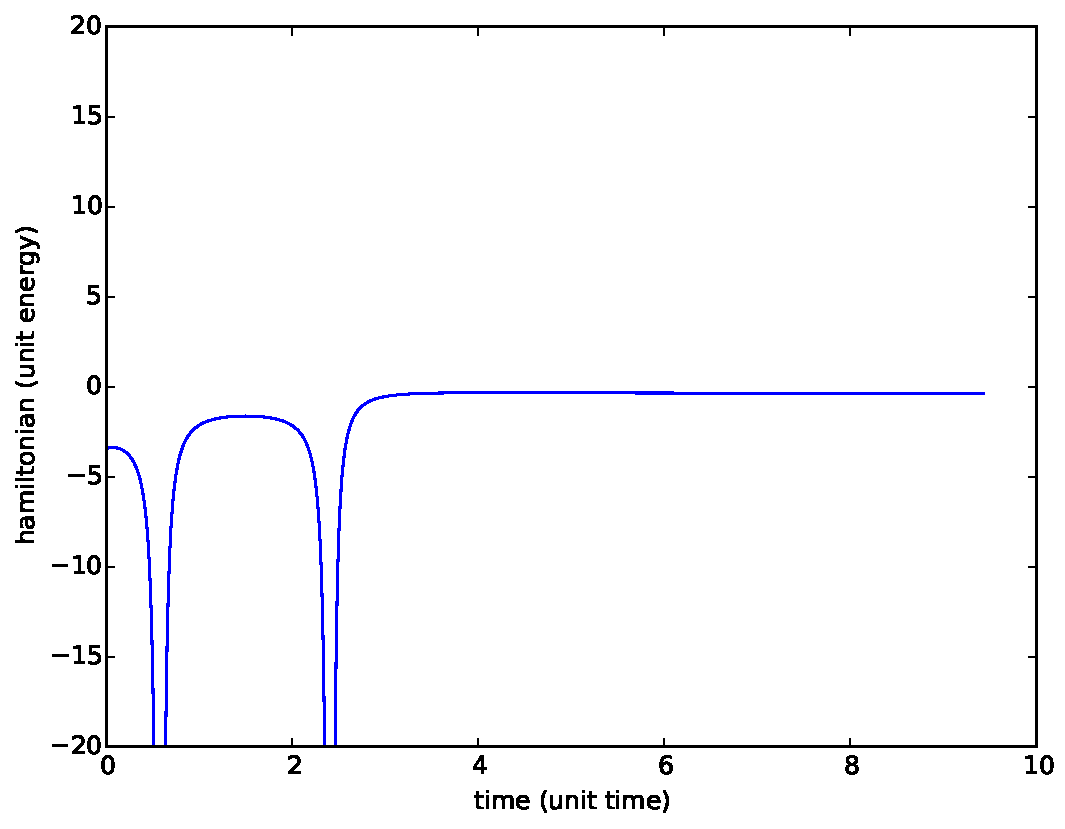
\includegraphics[scale=0.411]{fig/r3b-testing/r3b_H(t)_euler_explicit.pdf}
            \label{fig:r3b_H(t)_euler_explicit}
        }
        \caption{Explicit Euler trajectory and Hamiltonian. Ideally the $H(t)$ should be constant, but instead we see temporary dips for every Earth pass, and worse, the spacecraft picks up energy after every pass of Earth. Finally the spacecraft escapes the Earth with no apparent energy input. This is clearly wrong and not a valid trajectory}
        \label{fig:r3b_explicit_euler}
\end{figure}

\begin{figure}
    \centering
        \subbottom[Symplectic Euler $(\mathscr{X},\mathscr{Y})$ trajectory. Earth in origin, moon orbit in grey, first half of spacecraft trajectory is red, last half is blue.]{
            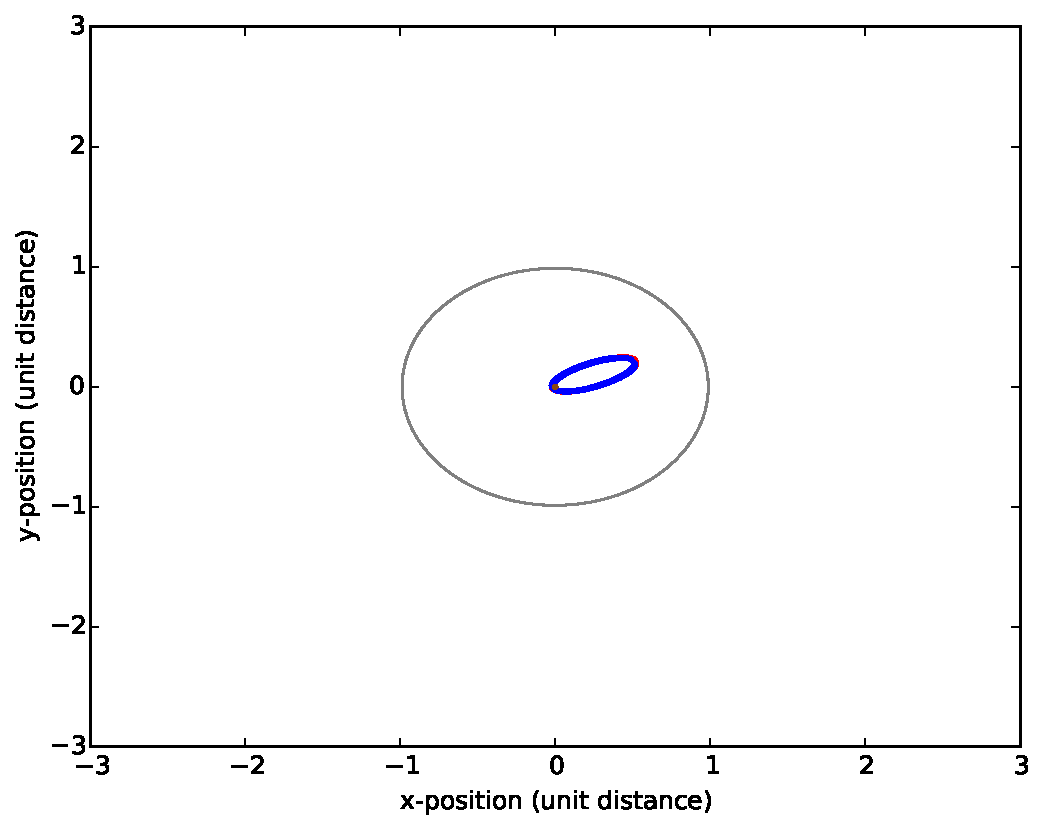
\includegraphics[scale=0.41]{fig/r3b-testing/r3b_y(x)_euler_symplectic.pdf}
            \label{fig:r3b_y(x)_euler_symplectic}
        }
        \subbottom[Symplectic Euler $H(t)$.]{
            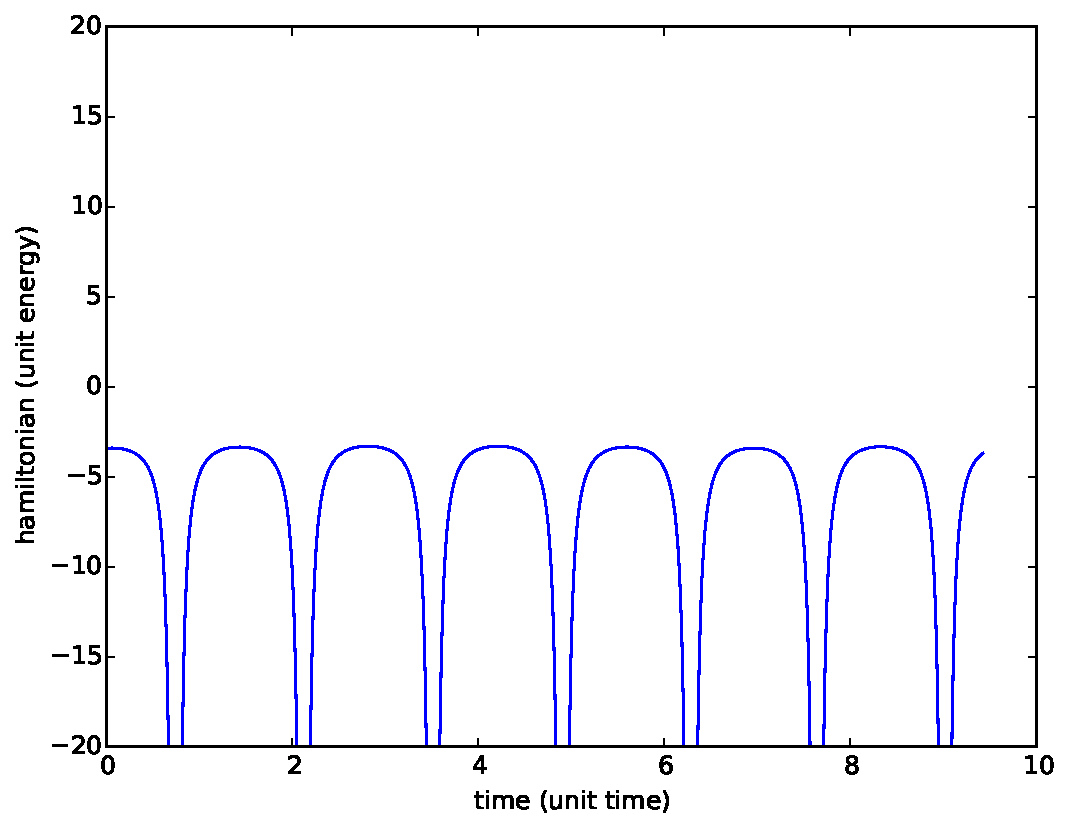
\includegraphics[scale=0.411]{fig/r3b-testing/r3b_H(t)_euler_symplectic.pdf}
            \label{fig:r3b_H(t)_euler_symplectic}
        }
        \caption{Symplectic Euler trajectory and Hamiltonian. The first half trajectory is red, the last half is blue. First we note the approximate elliptical orbit as expected. The $H(t)$ shows dips is the spacecraft passes the Earth, but on average over an orbit, $H(t)$ is approximately constant}
        \label{fig:r3b_symplectic_euler}
\end{figure}
Having $H$ conserved on average over an orbit is fine for a closed orbit, but for chaotic orbits around both Earth and Moon, it's not nearly good enough. We want a higher order method to conserve $H$ better, to better gauge the numerical errors, and to allow an adaptive numerical method.

Making the algorithm select a step size adaptively decreases the run time of a given simulation (though not necessarily the correctness of the solution). This is a big advantage because it allows us to search for many more orbits, which statistically will give us better orbits.

\section{Symplectic Störmer-Verlet}
We will now describe the second-order Störmer-Verlet method \cite{Hochbruck2008}:
\begin{align}
q_{i+1/2} &= q_i + \dfrac{h}{2}H_p(q_{i+1/2}, p_i), \\
p_{i+1} &= p_i + \dfrac{h}{2}(H_q(q_{i+1/2}, p_i) + H_q(q_{i+1/2}, p_{i+1})), \\
q_{i+1} &= q_{i+1/2} + \dfrac{h}{2}H_p(q_{n+1/2}, p_{i+1/2}).
\end{align}
where $H_q$ and $H_p$ denotes the partial derivatives of $H$, which can be expressed in terms of $q_i$ and $p_i$ by Hamilton's equations. Implemented for our equations (using~\cref{eq:H-x,eq:H-y,eq:H-px,eq:H-py} to express $H_q$ and $H_p$) we get:
\begin{align}
x_{i+1/2} &= (p_{x,i} + y_{i+1/2})\dfrac{h}{2} + x_i, \\[0.3cm]
y_{i+1/2} &= (p_{y,i} - x_{i+1/2})\dfrac{h}{2} + y_i, \\[0.8cm]
%
%
p_{x,i+1} &= \left[-H_{x,i} + (p_{x,i+1} + y_{i+1/2}) \right]\dfrac{h}{2} + p_{x,i}, \\[0.3cm]
%
p_{y,i+1} &= \left[-H_{y,i} + (p_{y,i+1} -x_{i+1/2}) \right]\dfrac{h}{2} + p_{y,i},\\[0.8cm]
%
%
x_{i+1} &= (p_{x,i+1} + y_{i+1/2})\dfrac{h}{2}, \\[0.3cm]
y_{i+1} &= (p_{y,i+1} - x_{i+1/2})\dfrac{h}{2},
\end{align}
where
\begin{align}
-H_{x,i} = \left(p_{y,i+1} - \dfrac{(1-k)(k+x_{i+1})}{((k+x_{i+1})^2+y_{i+1}^2)^{3/2}} + \dfrac{k(1-k-x_{i+1})}{((1-k-x_{i+1})^2+y_{i+1}^2)^{3/2}}\right), \\[0.5cm]
-H_{y,i} = \left(-p_{x,i+1} - \dfrac{(1-k)y_{i+1}}{((k+x_{i+1})^2+y_{i+1}^2)^{3/2}} - \dfrac{k y_{i+1}}{((1-k-x_{i+1})^2+y_{i+1}^2)^{3/2}}\right).
\end{align}


\section{Adaptive Symplectic Störmer-Verlet}
Let $z$ denote a vector of the position variables $(x,y)$.
\begin{align}
\text{Euler step result:} \qquad z_1 = z + O(h), \\
\text{Verlet step result:} \qquad z_2 = z + O(h^2), \\
\end{align}
where O(h) denotes an error term of order h. Then we take the difference
\begin{align}
\|z_1 - z_2\| &= O(h) - O(h^2) \\
&\approx O(h)\ ,
\end{align}
since $O(h) \gg O(h^2)$. Thus we approximate the error difference between the Euler and Verlet method as the actual error we make at step size $h$. The idea is to make both an Euler and a Verlet step for every time-step to assess the error and adjust the step size accordingly as implemented in listing \ref{lst:adaptive}
\begin{adjustwidth*}{0cm}{-0.4cm}
\begin{lstlisting}[language=Python,caption=Adaptive method implemented in python. We accept the Verlet step only if the error is no more than a given tolerance \texttt{tol}. Subsequently we estimate a new \texttt{h} that will yield an error of \texttt{tol} in the next step and use \texttt{0.8} of this value to avoid frequent rejects. If the step is rejected we reduce the step size by half,label=lst:adaptive]
if err < tol or h <= h_min:

    # Accept step
    x = x2
    y = y2
    px = px2
    py = py2

    # Forward time by step
    t = t+h
    h = max(h_min, h*max(0.1, 0.8*sqrt(tol/err)))

else:
    # No accept, reduce h to half
    h = max(h_min, 0.5*h)
\end{lstlisting}
\end{adjustwidth*}
For every single step the step size is changed either up or down, depending on the errors and tolerance. As a result we always stay near the same error in every step, only taking as small steps as necessary in each iteration.

The non-adaptive algorithm is fixed in step size but varies in error per step.
The adaptive algorithm varies in step size in an attempt to fix the error per step.

For all simulations we have set $10^{-9}$ as the maximum tolerated error per step in the adaptive algorithm. For the non-adaptive algorithm we select a fixed step size, $10^{-6}$, to ensure that it's reasonably low most of the time. For comparison a simulation was run with same initial conditions using the adaptive and non-adaptive algorithm, see Figure \ref{fig:non-adaptive-step_error} - \ref{fig:adaptive-step_error}. Position plot \ref{fig:adaptive-xy_XY} shown for completeness.

\begin{figure}
    \centering
        \subbottom[Non-adaptive symplectic Verlet step size.]{
            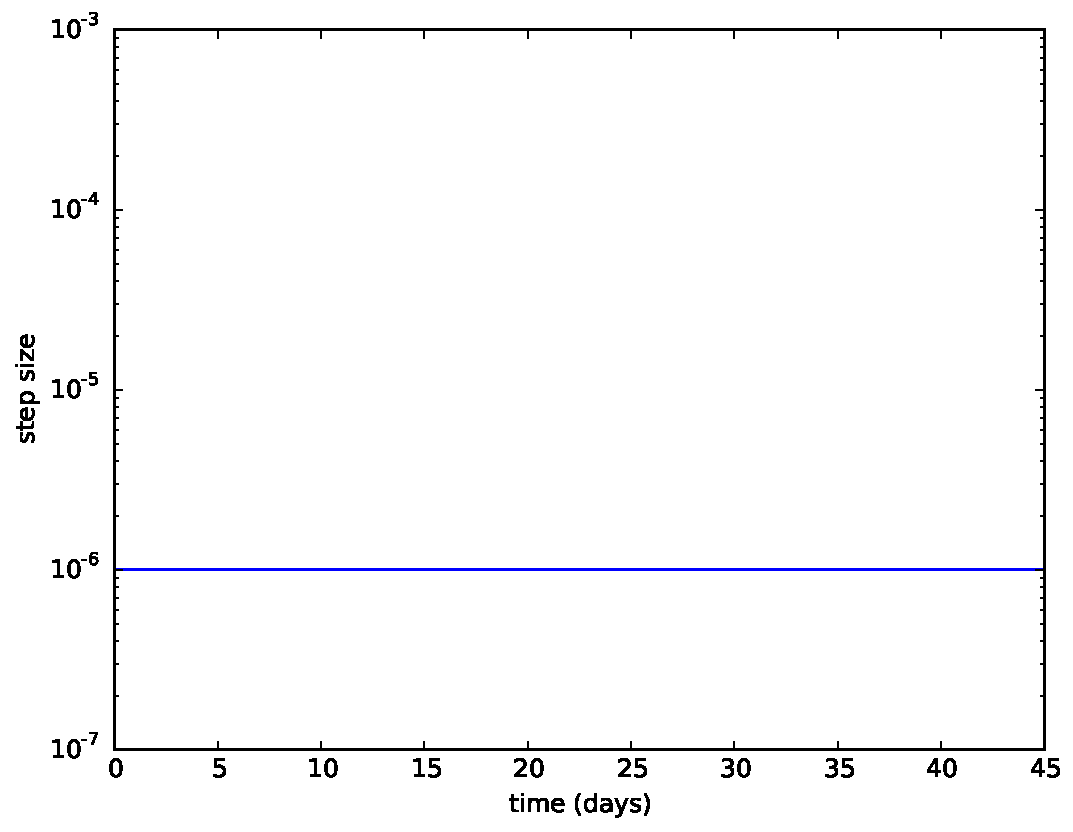
\includegraphics[scale=0.41]{fig/adaptive/step_fixed_h.pdf}
        }
        \subbottom[Non-adaptive symplectic Verlet error per step.]{
            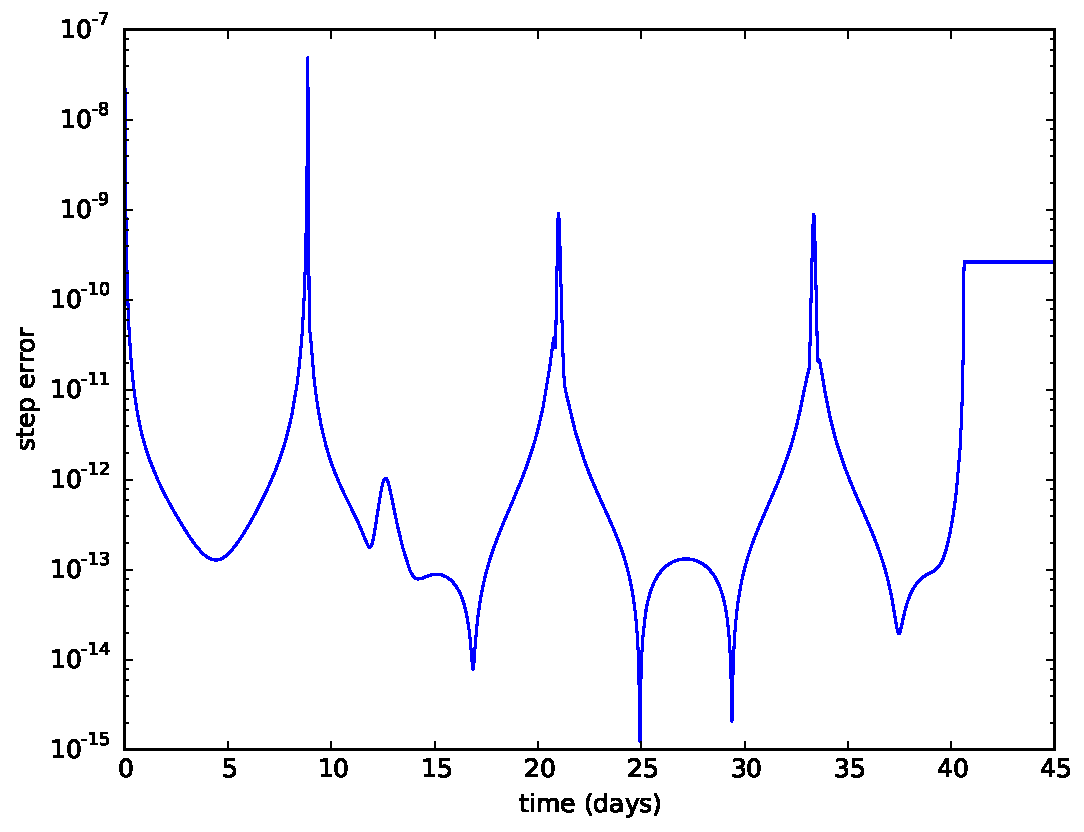
\includegraphics[scale=0.41]{fig/adaptive/err_fixed_h.pdf}
        \label{fig:non-adaptive-error}
        }
        \caption{Non-adaptive method step size and error per step. Step size is fixed and as a result the error varies. All the work spend on calculating the many steps with lower error than $10^{-9}$ in \ref{fig:non-adaptive-error} are wasted since the error spikes to somewhere $10^{-8}$ and $10^{-7}$ during a close fly-by, which might invalidate all decimals after the 7th decimal on the non-adaptive method. The solutions are practically identical, but the adaptive is much faster}
        \label{fig:non-adaptive-step_error}
\end{figure}


\begin{figure}
    \centering
        \subbottom[Adaptive symplectic Verlet step size.]{
            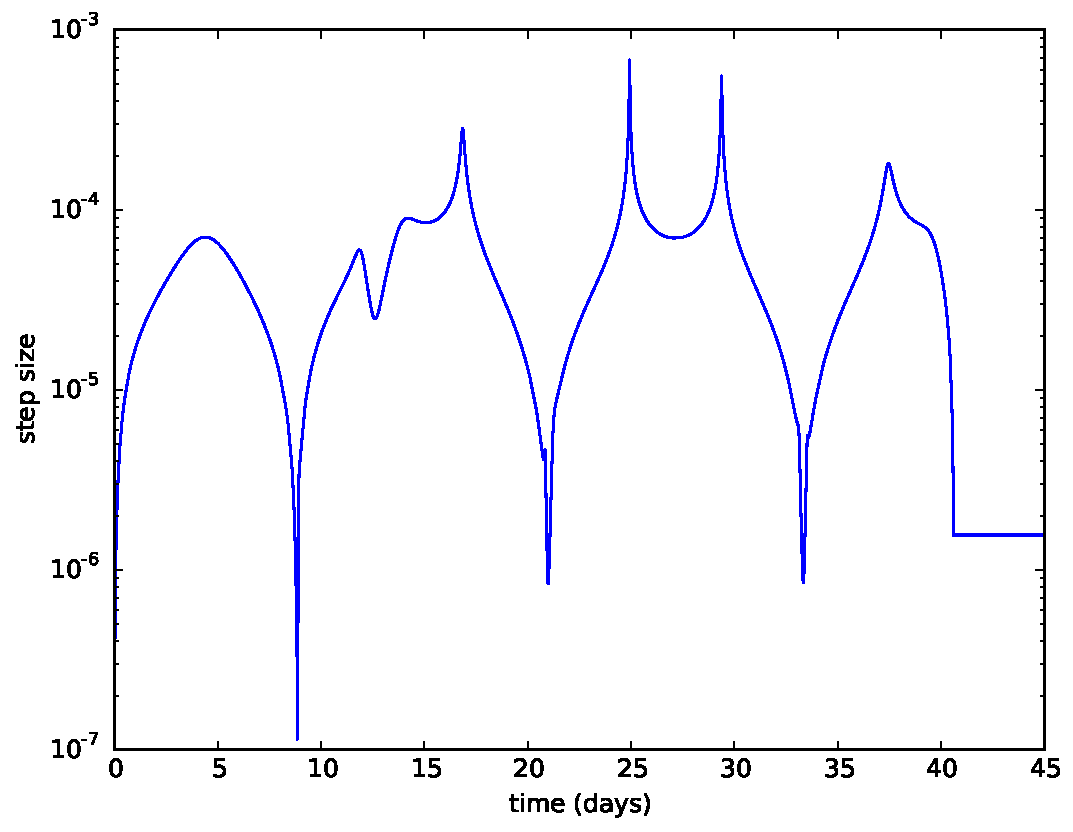
\includegraphics[scale=0.41]{fig/adaptive/step_adaptive.pdf}
        \label{fig:adaptive-step size}    
        }
        \subbottom[Adaptive symplectic Verlet error per step.]{
            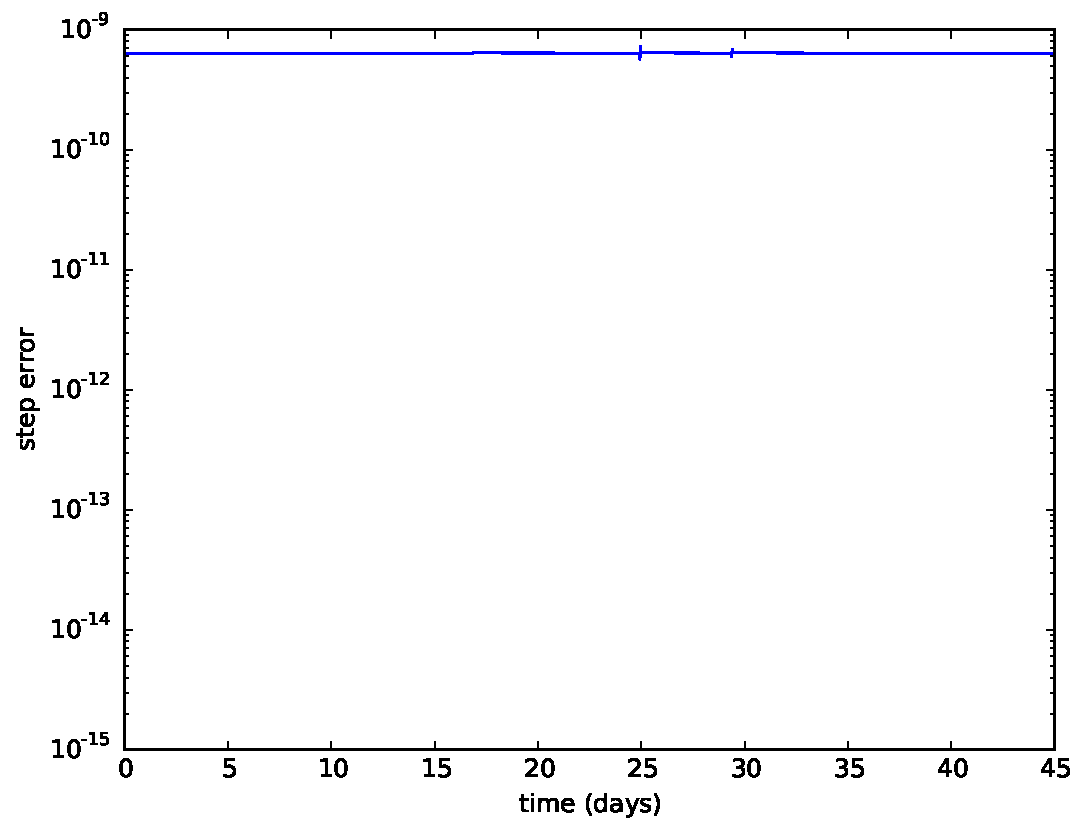
\includegraphics[scale=0.41]{fig/adaptive/err_adaptive.pdf}
        }
        \caption{The adaptive method constantly varies the step-size to ensure a constant error around $10^{-9}$. As a result it takes longer steps when there is less change in the variables, in the space far from the bodies, and shorter steps when passing close by the Earth or Moon}
        \label{fig:adaptive-step_error}
\end{figure}

\begin{figure}
    \centering
        \subbottom[Non-adaptive symplectic Verlet $(x,y)$ trajectory.]{
            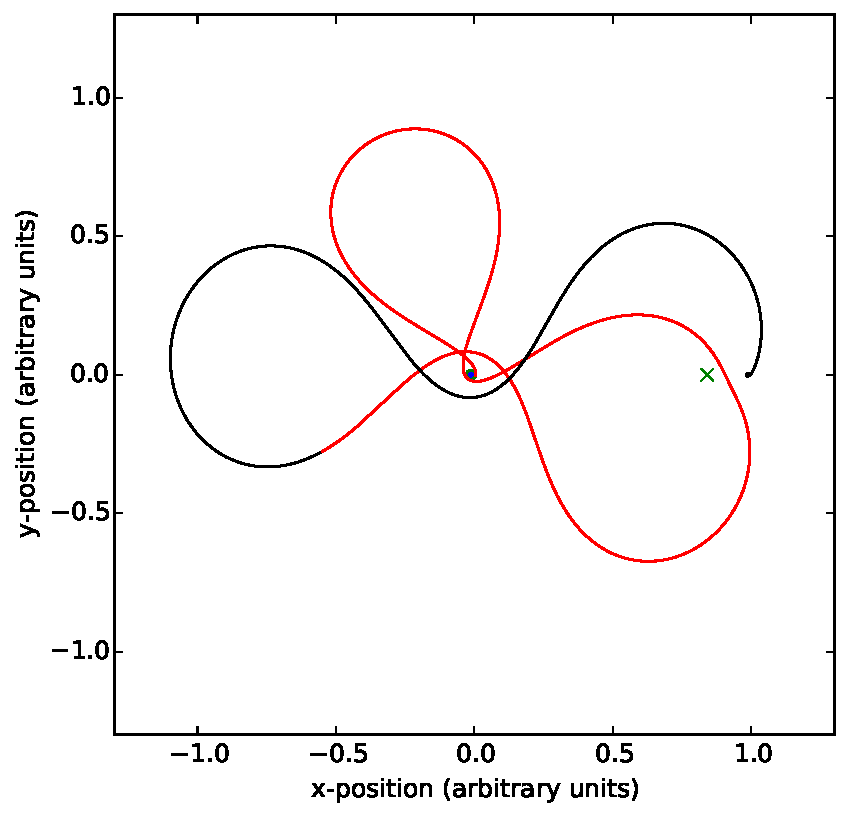
\includegraphics[scale=0.5]{fig/adaptive/_x-y_fixed_h.pdf}
        }
        \subbottom[Non-adaptive symplectic Verlet $(\mathscr{X},\mathscr{Y})$ trajectory.]{
            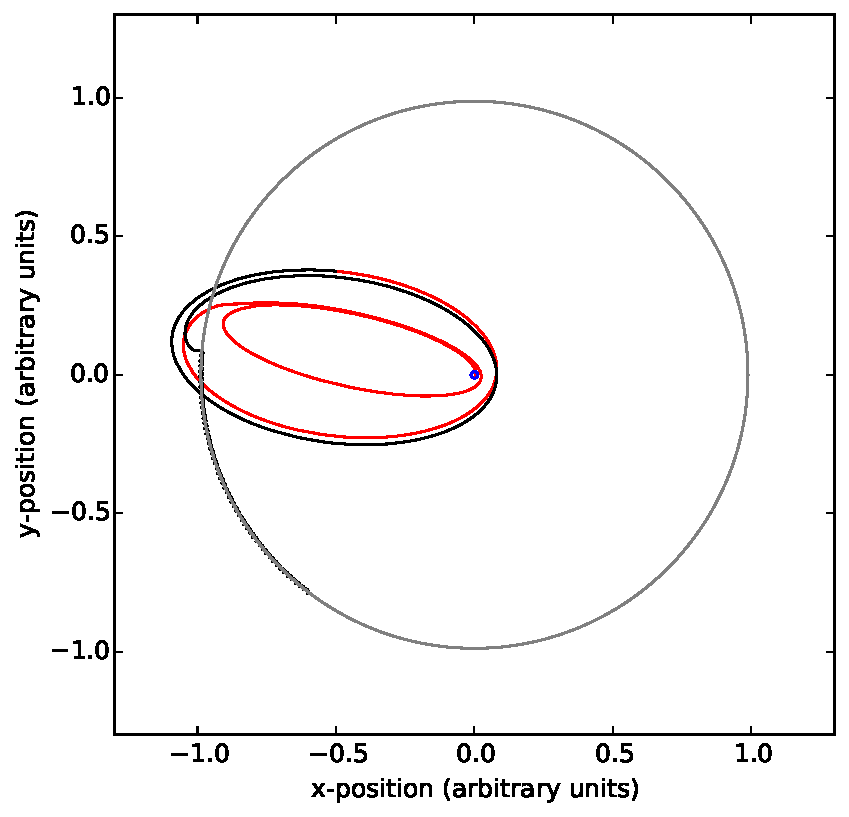
\includegraphics[scale=0.5]{fig/adaptive/X-Y_fixed_h.pdf}
        }
        \caption{The trajectories of same initial conditions for the adaptive and non-adaptive method was visually indistinguishable. Included for context to Figure \ref{fig:non-adaptive-step_error} - \ref{fig:adaptive-step_error}}
        \label{fig:adaptive-xy_XY}
\end{figure}


Note on the step size Figure \ref{fig:adaptive-step size} that the adaptive ends up with constant step size at the end at 40 days once captured by the Moon. Thus when we are in circular orbit around a single body, we don't gain much by using adaptive methods. However as the spacecraft are in free space far away from both Earth/Moon, we gain a lot by taking longer steps (raising the step size). However as we make close passes to Earth or Moon, then the step size dips sharply to maintain constant error. We see this around day 9, 21 and 33 in \ref{fig:adaptive-step size}. For most simulations, the adaptive method ran 10-100 times faster.

The code for the full Python implementation is in appendix \ref{app:code-r3b}.
